% ----------------------------------------------------------------------
% 13eme Colloque National en Calcul des Structures
% ----------------------------------------------------------------------
% 15-19 mai 2017, Presqu'ile de Giens
% ----------------------------------------------------------------------
\documentclass{CSMA2017}
% ----------------------------------------------------------------------
\title{13ème Colloque National \\ en Calcul des Structures}
% ----------------------------------------------------------------------
\author{V. Acary$^1$, M. Brémond$^2$, F. Dubois$^1$}
% ----------------------------------------------------------------------
\address{%
$^1$ INRIA. Grenoble, \{vincent.acary,maurice.bremond\}@inria.fr\\
$^2$ LMGC, Université de Montpellier, frederic.dubois@umontpellier.fr \\
}

% Mettre vos commandes personneles ici
% ----------------------------------------------------------------------
% Les commances \vect et \tens sont définies dans le fichier CSMA2017.cls




% ----------------------------------------------------------------------
\begin{document}
% ----------------------------------------------------------------------
\maketitle
% ----------------------------------------------------------------------

\begin{abstract}
Résumé de 6 lignes maximum. Résumé de 6 lignes maximum. Résumé de 6 lignes maximum. Résumé de 6 lignes maximum. Résumé de 6 lignes maximum. Résumé de 6 lignes maximum. Résumé de 6 lignes maximum. Résumé de 6 lignes maximum. Résumé de 6 lignes maximum. Résumé de 6 lignes maximum. Résumé de 6 lignes maximum. Résumé de 6 lignes maximum. Résumé de 6 lignes maximum. Résumé de 6 lignes maximum. Résumé de 6 lignes maximum. Résumé de 6 lignes maximum. Résumé de 6 lignes maximum. Résumé de 6 lignes maximum. Résumé de 6 lignes maximum.

\keywords mot clef1, mot clef2, mot clef3.
\end{abstract}

\section{Introduction}

\begin{itemize}
\item Description du problème de frottement discret
\item Problème de rang de H
\item Objectifs du papier
  \begin{enumerate}
  \item Comparaison performance NSGS/NSN sur des déformables et des rigides.
  \item Intérêt a passer en déformable pour ajouter des ddl.
  \end{enumerate}
\end{itemize}

\section{Méthodes numériques de résolution}

\section{Profils de perfomance}

\section{Comparaison sur des solides élastiques}

\subsection{La murette}
\subsection{Résultats}
\begin{figure}
  \centering
  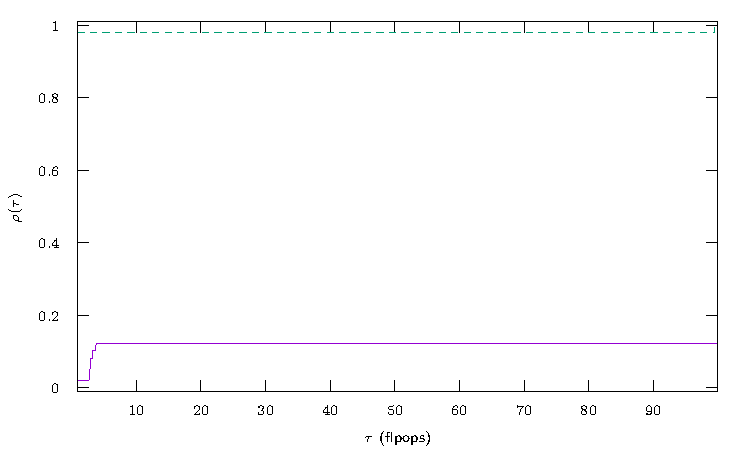
\includegraphics{figure/LowWall_FEM.1e-3/simple/profile-LMGC_LowWall_FEM.pdf}
  \includegraphics{figure/LowWall_FEM.1e-3/simple/profile-LMGC_LowWall_FEM_legend.pdf}
  \caption{Comparaison entre le solveur NSGS-AC et NSN-AC pour une précision de $10^{-3}$}
  \label{fig:LowWall_FEM.1e-3.simple}
\end{figure}
\begin{figure}
  \centering
  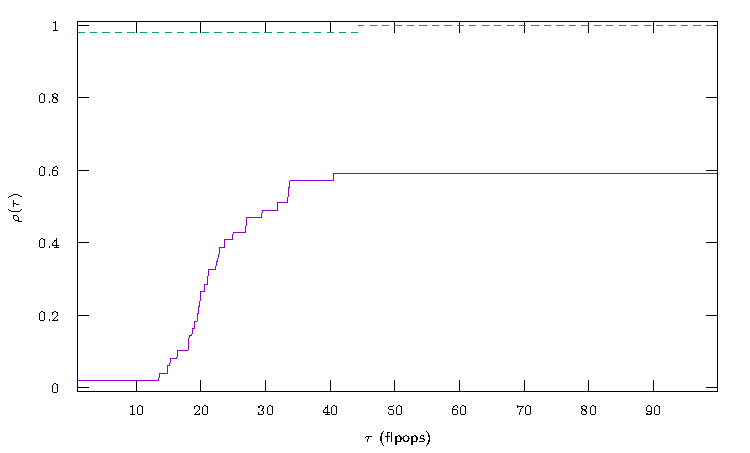
\includegraphics{figure/LowWall_FEM.1e-4/simple/profile-LMGC_LowWall_FEM.pdf}
  \includegraphics{figure/LowWall_FEM.1e-4/simple/profile-LMGC_LowWall_FEM_legend.pdf}
  \caption{Comparaison entre le solveur NSGS-AC et NSN-AC pour une précision de $10^{-4}$}
  \label{fig:LowWall_FEM.1e-4.simple}
\end{figure}
\begin{figure}
  \centering
  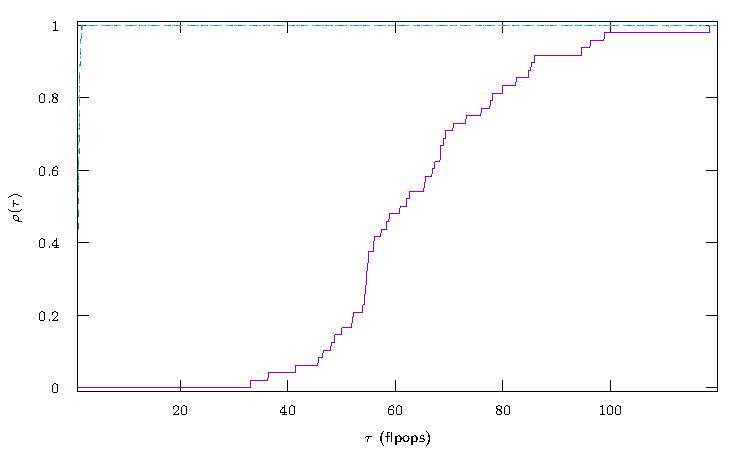
\includegraphics{figure/LowWall_FEM.1e-6/simple/profile-LMGC_LowWall_FEM.pdf}
  \includegraphics{figure/LowWall_FEM.1e-6/simple/profile-LMGC_LowWall_FEM_legend.pdf}
  \caption{Comparaison entre le solveur NSGS-AC et NSN-AC pour une précision de $10^{-6}$}
  \label{fig:LowWall_FEM.1e-6.simple}
\end{figure}


\begin{figure}
  \centering
  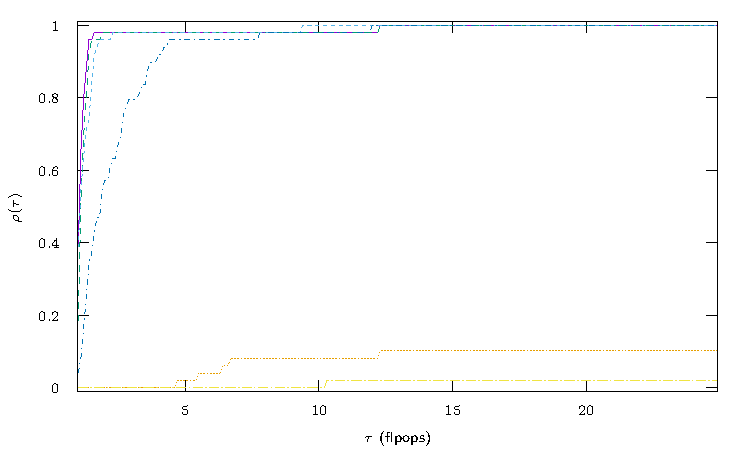
\includegraphics{figure/LowWall_FEM.1e-4/nsn_nls/profile-LMGC_LowWall_FEM.pdf}
  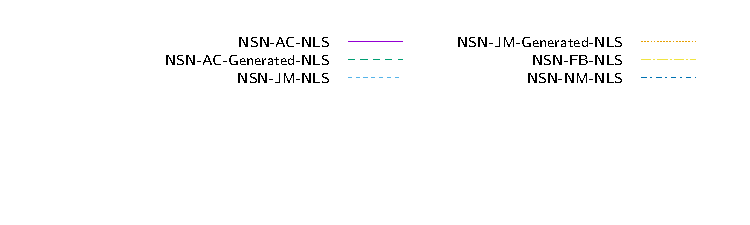
\includegraphics{figure/LowWall_FEM.1e-4/nsn_nls/profile-LMGC_LowWall_FEM_legend.pdf}
  \caption{Comparaison des solveurs NSN-*-NLS pour une précision de $10^{-4}$}
  \label{fig:LowWall_FEM.1e-4.nsn_nls}
\end{figure}
\begin{figure}
  \centering
  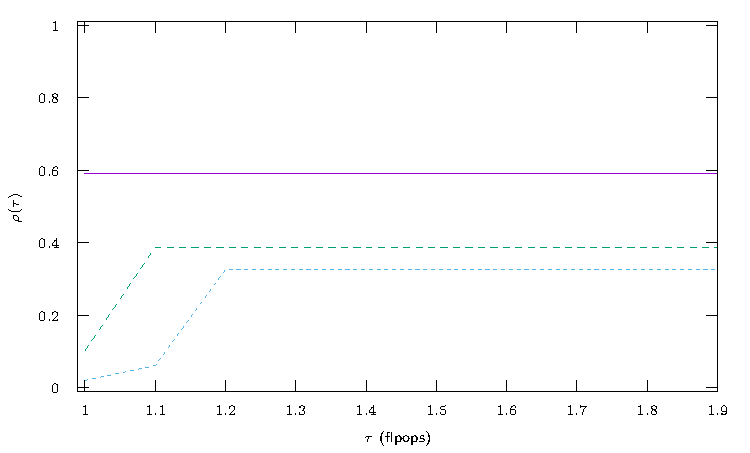
\includegraphics{figure/LowWall_FEM.1e-4/nsgs/profile-LMGC_LowWall_FEM.pdf}
  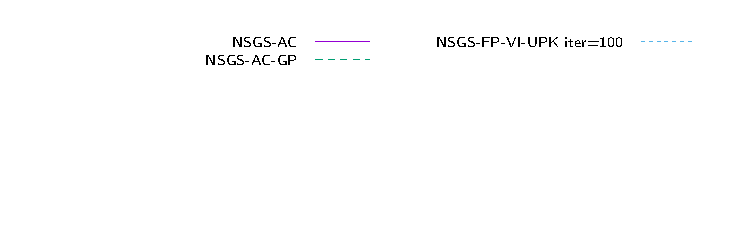
\includegraphics{figure/LowWall_FEM.1e-4/nsgs/profile-LMGC_LowWall_FEM_legend.pdf}
  \caption{Comparaison des solveurs NSGS pour une précision de $10^{-4}$}
  \label{fig:LowWall_FEM.1e-4.nsgs}
\end{figure}

\section{Comparaison sur des solides rigides}

\section{Utilisation des solides élastiques pour améliorer la convergence}

\section{Conclusion}

parralelisme.
\subsection{Références bibliographiques}

Les références sont à insérer en fin de document, numérotées par ordre alphabétique des auteurs. Trois exemples de références sont proposés : un article \cite{article} et un acte \cite{acte} et un livre  \cite{livre}.


% ----------------------------------------------------------------------
\begin{thebibliography}{1}
% ----------------------------------------------------------------------
\bibitem{article}
P. Auteur, D. Auteur, T. Auteur. \emph{Titre de l'article}, Revue, Éditeur, page1-pageN, Année. 
\bibitem{acte} P. Auteur. \emph{Titre de l'acte}, Titre de l'ouvrage, Éditeur, page1-pageN, Année.
\bibitem{livre} P. Auteur, D. Auteur. \emph{Titre de l'ouvrage}, Éditeur, Année. 

% ----------------------------------------------------------------------
\end{thebibliography}
% ----------------------------------------------------------------------

% ----------------------------------------------------------------------
\end{document}
% ----------------------------------------------------------------------
